\scanpage{52}
% E: margin note|top, continuation|dans chacun des arcs
\margin{\deleted{\unsure{NB}} dans chacun des arcs \deleted{\unsure{complémentaires}} déterminés par \(s,t\) sur \(\delta F\), il y a au moins un pt critique.}

% E: text|left upper, d|Relation entre sommets critiques
d) \uline{Relation entre} sommets critiques \deleted{\unsure{de}} sur \(F\) et sur \(F'=\sigma_a(F)\)

\(a\) un \uline{grand côté} sur \(\delta F\). OPS que \(\varepsilon_F(a)=1\) (quitte à intervertir les rôles de \(F\) et \(F'\)). On a deux cas :

% E: text|left upper-middle, definitions|Soit t l'antipodique
Soit \deleted{\unsure{\(s\) le pt critique sur \(a\)}}\inserted{\(t\) l'antipodique de \(s\), qui est critique}, \(u,v\) les deux pts critiques les plus voisins de \unsure{\(t\)|\(s\)} \deleted{de \(\delta F\)} de part et d'autre de \(s\), \(\beta=\widehat{\unsure{u^*tv^*|utv}}\) l'arc correspondant\inserted{de \(\delta F\)}, d'extrémités \(u,v\) contenant \(s\). Considérons \unsure{\(\beta\)}\inserted{l'autre} arc d'extrémités \(\unsure{u^*|u}\) et \(v^*\), soit \(\alpha\). \deleted{Soit} (NB, on a \(u,v\) sur deux arcs\inserted{ouverts} distincts déterminés par \(s,t\) sur \(\delta F\), \deleted{\unsure{et}} et \(u\ne v\), donc \unsure{\(s\in\)}\deleted{\(\beta\)}\inserted{\(\alpha\)}, de façon précise \(\alpha=\widehat{usv}\)). \deleted{\unsure{Donnons}} \(\unsure{s'=s},t',u',v'\) \deleted{\unsure{les}} transformés de \(s,t,u,v\) par \(\sigma_a\).

% E: drawing|left middle|two tangent ovals s t u v and primes
\figure{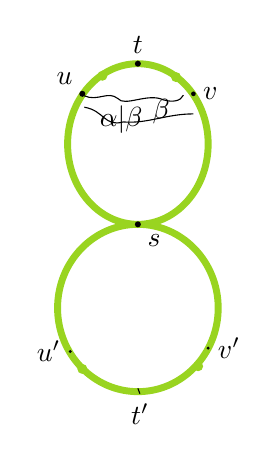
\begin{tikzpicture}[scale=.85]
\draw[yellow!60!green,line width=2.5pt] (0,1.25) ellipse (1.05 and 1.2) (0,-1.2) ellipse (1.2 and 1.25);
\fill (0,.05) circle(.045) node[below right] {$s$};
\fill (0,2.45) circle(.045) node[above] {$t$};
\fill (-.83,2) circle(.045) node[above left] {$u$};
\fill (.83,2) circle(.035) node[right] {$v$};
\fill (-1.01,-1.85) circle(.025) node[left] {$u'$};
\fill (1.05,-1.8) circle(.025) node[right] {$v'$};
\draw (0,-2.4)--(.03,-2.48) node[below] {$t'$};
\foreach \p in {(-.53,2.27),(.57,2.25),(-.83,-2.11),(.9,-2.07)}{\fill[yellow!60!green] \p circle(.075);}
\draw (-.8,1.97)..controls (-.6,1.88) and (-.45,2.05)..(-.3,1.93)..controls (-.2,1.8) and (.15,2.02)..(.38,1.91)..controls (.52,1.87) and (.64,1.89)..(.68,1.98);
\node at (.35,1.74) {$\beta$};
\draw (-.8,1.8)..controls (-.5,1.75) and (-.5,1.5)..(-.22,1.58)..controls (.15,1.55) and (.42,1.7)..(.83,1.7);
\node at (-.25,1.61) {$\deleted{\unsure{\alpha|\beta}}$};
\end{tikzpicture}}

% E: text|left middle-lower, a|sigma induit une bijection
Alors

a) \deleted{\unsure{\(C_K\)}} \uline{\(\sigma_a\) induit une bijection entre \(C_K\cap\alpha\) et \(C_K\cap\alpha'\)}.
\deleted{\unsure{Jeux induits, avec la condition ci-dessous, que}}
Si \(x\) et \(x'\) se correspondent par \(\sigma_a\), on a \(\varepsilon_F(x)=\varepsilon_{\unsure{F|F'}}(x')\), sauf si \(x=s\), donc \(x'=s\) (auquel cas \(\varepsilon_{F'}(x)=-\varepsilon_F(x)\)).

% E: text|left lower, b|On a t' non critique
b) On a \(t'\notin C_K\), \deleted{l'intersection} \(\operatorname{card}(\mathring{\beta}'\cap C_K)\)\deleted{\unsure{\(\leq2\)}}\(\in\{0,1,2\}\).
\inserted{Donc si l'ordre\inserted{\unsure{réduit}} de \(F\) resp. \(F'\) est \(N\) resp. \(N'\), on a \(N'\in\{N-1,N,N+1\}\)}
\deleted{\unsure{tout à}} Si \(x\in\mathring{\beta}'\cap C_K\), on a \(\varepsilon_F(x)=-1\).

% E: text|left bottom, corollary|Considérons les antipodiques
\uline{Cor} Considérons les antipodiques \(u^*,v^*\) de \(u,v\) sur \(\delta F\), et l'arc \(\beta^*=\widehat{u^*sv^*}\), \deleted{Alors} \unsure{dans|alors} son intérieur il n'y a pas de pts critiques de signe \(\unsure{\ne1|+1}\).

% E: text|right top, summary|En résumé
\uline{En résumé} Soit \(x\in S_K\cap\delta F\), \deleted{\unsure{un sommet de \(s\)}} \(x'=\sigma_a(\unsure{F|x})\), alors \(x'\) est critique ssi \(x\) l'est, et \(x\) et \(x'\) ont $=$ indice sauf dans les cas suivants

% E: display|right upper, a|x equals s
a) \(x=s\), auquel cas : \(\varepsilon_{F'}(x)=-\varepsilon_F(x')\)

% E: text|right upper-middle, b|x equals t
b) \(x=t\), auquel cas \deleted{\unsure{un}} \(\unsure{x|t}\) est critique d'indice \(+1\), \(\unsure{x''|x'}\) non critique

% E: text|right middle, parenthesis|Ceci permet de distinguer
(Ceci permet de distinguer \deleted{\unsure{quel}}\inserted{lequel} des deux faces \(F,F'\) est ``\deleted{\unsure{principale}}\inserted{\uline{\unsure{privilégié}}}'' par rapport à l'autre, en termes de la position de l'unique critique \(\unsure{s}\) sur \(a\), et ses \deleted{\unsure{deux}} antipodiques sur \(\delta F,\delta F'\))

% E: text|right lower, c|x in open arc
c) \(x\in\mathring{\widehat{utv}}=\mathring{\beta}\), avec \(x\ne t\)

i.e. \(x'\ne t'\), alors \(x\) non critique, alors il peut exister 1 ou 2 cas (au maximum) tels que \(x'\) soit critique --- son indice est alors \(-1\).
\mspage{51}
